
%% bare_jrnl.tex
%% V1.3
%% 2007/01/11
%% by Michael Shell
%% see http://www.michaelshell.org/
%% for current contact information.
%%
%% This is a skeleton file demonstrating the use of IEEEtran.cls
%% (requires IEEEtran.cls version 1.7 or later) with an IEEE journal paper.
%%
%% Support sites:
%% http://www.michaelshell.org/tex/ieeetran/
%% http://www.ctan.org/tex-archive/macros/latex/contrib/IEEEtran/
%% and
%% http://www.ieee.org/



% *** Authors should verify (and, if needed, correct) their LaTeX system  ***
% *** with the testflow diagnostic prior to trusting their LaTeX platform ***
% *** with production work. IEEE's font choices can trigger bugs that do  ***
% *** not appear when using other class files.                            ***
% The testflow support page is at:
% http://www.michaelshell.org/tex/testflow/


%%*************************************************************************
%% Legal Notice:
%% This code is offered as-is without any warranty either expressed or
%% implied; without even the implied warranty of MERCHANTABILITY or
%% FITNESS FOR A PARTICULAR PURPOSE! 
%% User assumes all risk.
%% In no event shall IEEE or any contributor to this code be liable for
%% any damages or losses, including, but not limited to, incidental,
%% consequential, or any other damages, resulting from the use or misuse
%% of any information contained here.
%%
%% All comments are the opinions of their respective authors and are not
%% necessarily endorsed by the IEEE.
%%
%% This work is distributed under the LaTeX Project Public License (LPPL)
%% ( http://www.latex-project.org/ ) version 1.3, and may be freely used,
%% distributed and modified. A copy of the LPPL, version 1.3, is included
%% in the base LaTeX documentation of all distributions of LaTeX released
%% 2003/12/01 or later.
%% Retain all contribution notices and credits.
%% ** Modified files should be clearly indicated as such, including  **
%% ** renaming them and changing author support contact information. **
%%
%% File list of work: IEEEtran.cls, IEEEtran_HOWTO.pdf, bare_adv.tex,
%%                    bare_conf.tex, bare_jrnl.tex, bare_jrnl_compsoc.tex
%%*************************************************************************

% Note that the a4paper option is mainly intended so that authors in
% countries using A4 can easily print to A4 and see how their papers will
% look in print - the typesetting of the document will not typically be
% affected with changes in paper size (but the bottom and side margins will).
% Use the testflow package mentioned above to verify correct handling of
% both paper sizes by the user's LaTeX system.
%
% Also note that the "draftcls" or "draftclsnofoot", not "draft", option
% should be used if it is desired that the figures are to be displayed in
% draft mode.
%
\documentclass[journal]{IEEEtran}
%
% If IEEEtran.cls has not been installed into the LaTeX system files,
% manually specify the path to it like:
% \documentclass[journal]{../sty/IEEEtran}





% Some very useful LaTeX packages include:
% (uncomment the ones you want to load)


% *** MISC UTILITY PACKAGES ***
%
%\usepackage{ifpdf}
% Heiko Oberdiek's ifpdf.sty is very useful if you need conditional
% compilation based on whether the output is pdf or dvi.
% usage:
% \ifpdf
%   % pdf code
% \else
%   % dvi code
% \fi
% The latest version of ifpdf.sty can be obtained from:
% http://www.ctan.org/tex-archive/macros/latex/contrib/oberdiek/
% Also, note that IEEEtran.cls V1.7 and later provides a builtin
% \ifCLASSINFOpdf conditional that works the same way.
% When switching from latex to pdflatex and vice-versa, the compiler may
% have to be run twice to clear warning/error messages.






% *** CITATION PACKAGES ***
%
\usepackage{cite}
% cite.sty was written by Donald Arseneau
% V1.6 and later of IEEEtran pre-defines the format of the cite.sty package
% \cite{} output to follow that of IEEE. Loading the cite package will
% result in citation numbers being automatically sorted and properly
% "compressed/ranged". e.g., [1], [9], [2], [7], [5], [6] without using
% cite.sty will become [1], [2], [5]--[7], [9] using cite.sty. cite.sty's
% \cite will automatically add leading space, if needed. Use cite.sty's
% noadjust option (cite.sty V3.8 and later) if you want to turn this off.
% cite.sty is already installed on most LaTeX systems. Be sure and use
% version 4.0 (2003-05-27) and later if using hyperref.sty. cite.sty does
% not currently provide for hyperlinked citations.
% The latest version can be obtained at:
% http://www.ctan.org/tex-archive/macros/latex/contrib/cite/
% The documentation is contained in the cite.sty file itself.






% *** GRAPHICS RELATED PACKAGES ***
%
\ifCLASSINFOpdf
  \usepackage[pdftex]{graphicx}
  % declare the path(s) where your graphic files are
  \graphicspath{{img/}}
  % and their extensions so you won't have to specify these with
  % every instance of \includegraphics
  \DeclareGraphicsExtensions{.pdf,.jpeg,.png}
\else
  % or other class option (dvipsone, dvipdf, if not using dvips). graphicx
  % will default to the driver specified in the system graphics.cfg if no
  % driver is specified.
  % \usepackage[dvips]{graphicx}
  % declare the path(s) where your graphic files are
  % \graphicspath{{../eps/}}
  % and their extensions so you won't have to specify these with
  % every instance of \includegraphics
  % \DeclareGraphicsExtensions{.eps}
\fi
% graphicx was written by David Carlisle and Sebastian Rahtz. It is
% required if you want graphics, photos, etc. graphicx.sty is already
% installed on most LaTeX systems. The latest version and documentation can
% be obtained at: 
% http://www.ctan.org/tex-archive/macros/latex/required/graphics/
% Another good source of documentation is "Using Imported Graphics in
% LaTeX2e" by Keith Reckdahl which can be found as epslatex.ps or
% epslatex.pdf at: http://www.ctan.org/tex-archive/info/
%
% latex, and pdflatex in dvi mode, support graphics in encapsulated
% postscript (.eps) format. pdflatex in pdf mode supports graphics
% in .pdf, .jpeg, .png and .mps (metapost) formats. Users should ensure
% that all non-photo figures use a vector format (.eps, .pdf, .mps) and
% not a bitmapped formats (.jpeg, .png). IEEE frowns on bitmapped formats
% which can result in "jaggedy"/blurry rendering of lines and letters as
% well as large increases in file sizes.
%
% You can find documentation about the pdfTeX application at:
% http://www.tug.org/applications/pdftex





% *** MATH PACKAGES ***
%
\usepackage{amsmath, amssymb , amsthm}
% A popular package from the American Mathematical Society that provides
% many useful and powerful commands for dealing with mathematics. If using
% it, be sure to load this package with the cmex10 option to ensure that
% only type 1 fonts will utilized at all point sizes. Without this option,
% it is possible that some math symbols, particularly those within
% footnotes, will be rendered in bitmap form which will result in a
% document that can not be IEEE Xplore compliant!
%
% Also, note that the amsmath package sets \interdisplaylinepenalty to 10000
% thus preventing page breaks from occurring within multiline equations. Use:
%\interdisplaylinepenalty=2500
% after loading amsmath to restore such page breaks as IEEEtran.cls normally
% does. amsmath.sty is already installed on most LaTeX systems. The latest
% version and documentation can be obtained at:
% http://www.ctan.org/tex-archive/macros/latex/required/amslatex/math/





% *** SPECIALIZED LIST PACKAGES ***
%
%\usepackage{algorithmic}
% algorithmic.sty was written by Peter Williams and Rogerio Brito.
% This package provides an algorithmic environment fo describing algorithms.
% You can use the algorithmic environment in-text or within a figure
% environment to provide for a floating algorithm. Do NOT use the algorithm
% floating environment provided by algorithm.sty (by the same authors) or
% algorithm2e.sty (by Christophe Fiorio) as IEEE does not use dedicated
% algorithm float types and packages that provide these will not provide
% correct IEEE style captions. The latest version and documentation of
% algorithmic.sty can be obtained at:
% http://www.ctan.org/tex-archive/macros/latex/contrib/algorithms/
% There is also a support site at:
% http://algorithms.berlios.de/index.html
% Also of interest may be the (relatively newer and more customizable)
% algorithmicx.sty package by Szasz Janos:
% http://www.ctan.org/tex-archive/macros/latex/contrib/algorithmicx/




% *** ALIGNMENT PACKAGES ***
%
\usepackage{array}
% Frank Mittelbach's and David Carlisle's array.sty patches and improves
% the standard LaTeX2e array and tabular environments to provide better
% appearance and additional user controls. As the default LaTeX2e table
% generation code is lacking to the point of almost being broken with
% respect to the quality of the end results, all users are strongly
% advised to use an enhanced (at the very least that provided by array.sty)
% set of table tools. array.sty is already installed on most systems. The
% latest version and documentation can be obtained at:
% http://www.ctan.org/tex-archive/macros/latex/required/tools/


\usepackage{mdwmath}
\usepackage{mdwtab}
% Also highly recommended is Mark Wooding's extremely powerful MDW tools,
% especially mdwmath.sty and mdwtab.sty which are used to format equations
% and tables, respectively. The MDWtools set is already installed on most
% LaTeX systems. The lastest version and documentation is available at:
% http://www.ctan.org/tex-archive/macros/latex/contrib/mdwtools/


% IEEEtran contains the IEEEeqnarray family of commands that can be used to
% generate multiline equations as well as matrices, tables, etc., of high
% quality.


%\usepackage{eqparbox}
% Also of notable interest is Scott Pakin's eqparbox package for creating
% (automatically sized) equal width boxes - aka "natural width parboxes".
% Available at:
% http://www.ctan.org/tex-archive/macros/latex/contrib/eqparbox/





% *** SUBFIGURE PACKAGES ***
%\usepackage[tight,footnotesize]{subfigure}
% subfigure.sty was written by Steven Douglas Cochran. This package makes it
% easy to put subfigures in your figures. e.g., "Figure 1a and 1b". For IEEE
% work, it is a good idea to load it with the tight package option to reduce
% the amount of white space around the subfigures. subfigure.sty is already
% installed on most LaTeX systems. The latest version and documentation can
% be obtained at:
% http://www.ctan.org/tex-archive/obsolete/macros/latex/contrib/subfigure/
% subfigure.sty has been superceeded by subfig.sty.



%\usepackage[caption=false]{caption}
%\usepackage[font=footnotesize]{subfig}
% subfig.sty, also written by Steven Douglas Cochran, is the modern
% replacement for subfigure.sty. However, subfig.sty requires and
% automatically loads Axel Sommerfeldt's caption.sty which will override
% IEEEtran.cls handling of captions and this will result in nonIEEE style
% figure/table captions. To prevent this problem, be sure and preload
% caption.sty with its "caption=false" package option. This is will preserve
% IEEEtran.cls handing of captions. Version 1.3 (2005/06/28) and later 
% (recommended due to many improvements over 1.2) of subfig.sty supports
% the caption=false option directly:
%\usepackage[caption=false,font=footnotesize]{subfig}
%
% The latest version and documentation can be obtained at:
% http://www.ctan.org/tex-archive/macros/latex/contrib/subfig/
% The latest version and documentation of caption.sty can be obtained at:
% http://www.ctan.org/tex-archive/macros/latex/contrib/caption/




% *** FLOAT PACKAGES ***
%
%\usepackage{fixltx2e}
% fixltx2e, the successor to the earlier fix2col.sty, was written by
% Frank Mittelbach and David Carlisle. This package corrects a few problems
% in the LaTeX2e kernel, the most notable of which is that in current
% LaTeX2e releases, the ordering of single and double column floats is not
% guaranteed to be preserved. Thus, an unpatched LaTeX2e can allow a
% single column figure to be placed prior to an earlier double column
% figure. The latest version and documentation can be found at:
% http://www.ctan.org/tex-archive/macros/latex/base/



%\usepackage{stfloats}
% stfloats.sty was written by Sigitas Tolusis. This package gives LaTeX2e
% the ability to do double column floats at the bottom of the page as well
% as the top. (e.g., "\begin{figure*}[!b]" is not normally possible in
% LaTeX2e). It also provides a command:
%\fnbelowfloat
% to enable the placement of footnotes below bottom floats (the standard
% LaTeX2e kernel puts them above bottom floats). This is an invasive package
% which rewrites many portions of the LaTeX2e float routines. It may not work
% with other packages that modify the LaTeX2e float routines. The latest
% version and documentation can be obtained at:
% http://www.ctan.org/tex-archive/macros/latex/contrib/sttools/
% Documentation is contained in the stfloats.sty comments as well as in the
% presfull.pdf file. Do not use the stfloats baselinefloat ability as IEEE
% does not allow \baselineskip to stretch. Authors submitting work to the
% IEEE should note that IEEE rarely uses double column equations and
% that authors should try to avoid such use. Do not be tempted to use the
% cuted.sty or midfloat.sty packages (also by Sigitas Tolusis) as IEEE does
% not format its papers in such ways.


%\ifCLASSOPTIONcaptionsoff
%  \usepackage[nomarkers]{endfloat}
% \let\MYoriglatexcaption\caption
% \renewcommand{\caption}[2][\relax]{\MYoriglatexcaption[#2]{#2}}
%\fi
% endfloat.sty was written by James Darrell McCauley and Jeff Goldberg.
% This package may be useful when used in conjunction with IEEEtran.cls'
% captionsoff option. Some IEEE journals/societies require that submissions
% have lists of figures/tables at the end of the paper and that
% figures/tables without any captions are placed on a page by themselves at
% the end of the document. If needed, the draftcls IEEEtran class option or
% \CLASSINPUTbaselinestretch interface can be used to increase the line
% spacing as well. Be sure and use the nomarkers option of endfloat to
% prevent endfloat from "marking" where the figures would have been placed
% in the text. The two hack lines of code above are a slight modification of
% that suggested by in the endfloat docs (section 8.3.1) to ensure that
% the full captions always appear in the list of figures/tables - even if
% the user used the short optional argument of \caption[]{}.
% IEEE papers do not typically make use of \caption[]'s optional argument,
% so this should not be an issue. A similar trick can be used to disable
% captions of packages such as subfig.sty that lack options to turn off
% the subcaptions:
% For subfig.sty:
% \let\MYorigsubfloat\subfloat
% \renewcommand{\subfloat}[2][\relax]{\MYorigsubfloat[]{#2}}
% For subfigure.sty:
% \let\MYorigsubfigure\subfigure
% \renewcommand{\subfigure}[2][\relax]{\MYorigsubfigure[]{#2}}
% However, the above trick will not work if both optional arguments of
% the \subfloat/subfig command are used. Furthermore, there needs to be a
% description of each subfigure *somewhere* and endfloat does not add
% subfigure captions to its list of figures. Thus, the best approach is to
% avoid the use of subfigure captions (many IEEE journals avoid them anyway)
% and instead reference/explain all the subfigures within the main caption.
% The latest version of endfloat.sty and its documentation can obtained at:
% http://www.ctan.org/tex-archive/macros/latex/contrib/endfloat/
%
% The IEEEtran \ifCLASSOPTIONcaptionsoff conditional can also be used
% later in the document, say, to conditionally put the References on a 
% page by themselves.





% *** PDF, URL AND HYPERLINK PACKAGES ***
%
%\usepackage{url}
% url.sty was written by Donald Arseneau. It provides better support for
% handling and breaking URLs. url.sty is already installed on most LaTeX
% systems. The latest version can be obtained at:
% http://www.ctan.org/tex-archive/macros/latex/contrib/misc/
% Read the url.sty source comments for usage information. Basically,
% \url{my_url_here}.





% *** Do not adjust lengths that control margins, column widths, etc. ***
% *** Do not use packages that alter fonts (such as pslatex).         ***
% There should be no need to do such things with IEEEtran.cls V1.6 and later.
% (Unless specifically asked to do so by the journal or conference you plan
% to submit to, of course. )


% correct bad hyphenation here
\hyphenation{op-tical net-works semi-conduc-tor}


\begin{document}
%
% paper title
% can use linebreaks \\ within to get better formatting as desired
\title{Dimensionality Estimation of Datasets}
%
%
% author names and IEEE memberships
% note positions of commas and nonbreaking spaces ( ~ ) LaTeX will not break
% a structure at a ~ so this keeps an author's name from being broken across
% two lines.
% use \thanks{} to gain access to the first footnote area
% a separate \thanks must be used for each paragraph as LaTeX2e's \thanks
% was not built to handle multiple paragraphs
%

\author{Fahad Ashraf}% <-this % stops a space

% note the % following the last \IEEEmembership and also \thanks - 
% these prevent an unwanted space from occurring between the last author name
% and the end of the author line. i.e., if you had this:
% 
% \author{....lastname \thanks{...} \thanks{...} }
%                     ^------------^------------^----Do not want these spaces!
%
% a space would be appended to the last name and could cause every name on that
% line to be shifted left slightly. This is one of those "LaTeX things". For
% instance, "\textbf{A} \textbf{B}" will typeset as "A B" not "AB". To get
% "AB" then you have to do: "\textbf{A}\textbf{B}"
% \thanks is no different in this regard, so shield the last } of each \thanks
% that ends a line with a % and do not let a space in before the next \thanks.
% Spaces after \IEEEmembership other than the last one are OK (and needed) as
% you are supposed to have spaces between the names. For what it is worth,
% this is a minor point as most people would not even notice if the said evil
% space somehow managed to creep in.



% The paper headers
\markboth{Seminar: Embedded Systems and Robotics 2019/20, RRLAB, University of Kaiserslautern}%
{}
% The only time the second header will appear is for the odd numbered pages
% after the title page when using the twoside option.
% 







% make the title area
\maketitle


\begin{abstract}
%\boldmath
Dimensionality estimations of datasets is an important problem in the field of pattern recognition and knowledge discovery.
 In this paper, different methods for estimating intrinsic dimensionality are discussed with focus on global methods specifically 
 fractal-based methods.  A fractal-based approach using the Grassberger-Procaccia (GP) algorithm is discussed and as the GP algorithm doesn't
 preform well on high dimensionality datasets, an empirical procedure that improves the orignal alogrithm has been described.
\end{abstract}
% IEEEtran.cls defaults to using nonbold math in the Abstract.
% This preserves the distinction between vectors and scalars. However,
% if the journal you are submitting to favors bold math in the abstract,
% then you can use LaTeX's standard command \boldmath at the very start
% of the abstract to achieve this. Many IEEE journals frown on math
% in the abstract anyway.

% Note that keywords are not normally used for peerreview papers.
%\begin{IEEEkeywords}
%IEEEtran, journal, \LaTeX, paper, template.
%\end{IEEEkeywords}






% For peer review papers, you can put extra information on the cover
% page as needed:
% \ifCLASSOPTIONpeerreview
% \begin{center} \bfseries EDICS Category: 3-BBND \end{center}
% \fi
%
% For peerreview papers, this IEEEtran command inserts a page break and
% creates the second title. It will be ignored for other modes.
\IEEEpeerreviewmaketitle



\section{Introduction}
% The very first letter is a 2 line initial drop letter followed
% by the rest of the first word in caps.
% 
% form to use if the first word consists of a single letter:
% \IEEEPARstart{A}{demo} file is ....
% 
% form to use if you need the single drop letter followed by
% normal text (unknown if ever used by IEEE):
% \IEEEPARstart{A}{}demo file is ....
% 
% Some journals put the first two words in caps:
% \IEEEPARstart{T}{his demo} file is ....
% 
% Here we have the typical use of a "T" for an initial drop letter
% and "HIS" in caps to complete the first word.
\IEEEPARstart{I}{n} pattern recognition problems, data is represented as vectors 
of dimension \(d\). The data is then embedded in the vector space \( \mathbb{R}^d \) 
but this does not mean that the intrinsic dimensionality (ID) of the dataset is \(d\). 
The ID of a data set is the minimum number of free variables needed to represent the data without information 
loss. 

% You must have at least 2 lines in the paragraph with the drop letter
% (should never be an issue)



% \subsection{Subsection Heading Here}
% Subsection text here. If you want to cite something you can use the \verb \cite{key} command to create a reference.
% The command \verb \cite{Hillenbrand07} will create the reference \cite{Hillenbrand07} for you and the item will be automatically added to the REFERENCES section.
% To add new papers, books etc. you have to edit the agrosy.bib file.

% needed in second column of first page if using \IEEEpubid
%\IEEEpubidadjcol

% \subsubsection{Subsubsection Heading Here}
% Subsubsection text here.


\section{Local Methods}
Local methods try to estimate the topological dimension of the
data manifold. The definition of topological dimension was given by Brouwer
\cite{Brouwer75} in 1913. Topological dimension is the basis dimension of the local linear
approximation of the hypersurface on which the data resides, i.e. the tangent
space. The topological dimension is the number of dimensions of the tangent space at each point.
For example, a sphear has a two-dimensional tangent space that can also be viewd as a two-dimensional manifold
 and since the ID of a sphear is three, the topological dimension represent the lower bound of ID. 
Sometimes the topological is simply called local dimension, this is why the methods which estimate topological dimensions are 
called local methods. 
The basic algorithm to estimate the topological 
dimension was proposed by Fukunaga and Olsen \cite{Fukunaga76}. Other approaches 
to the Fukunaga-Olsen’s algorithm have been proposed to estimate locally 
ID. Among them the Near Neighbor Algorithm \cite{Pettis79} and the methods based on 
Topological Representing Networks (TRN) \cite{Martinetz94}.

\subsection{Fukunaga-Olsen’s algorithm}

The alogrithm is based on the observation that for the vectors embedded in a linear subspace, 
the dimension is equal to the number of non-zero eigenvalues of the covariance matrix. 
The basic idea of the algorithm is to examine the data in many small subregions and from this estimate 
the intrinsic dimensionality. For each region the eigenvalues of the local convariance matrix are computed. 
Then, The eigenvalues are normalized by dividing them by the largest eigenvalue. The intrinsic dimensionality is 
then defined as the number of normalized eigenvalues that are larger that a threshold \(T\). The values \(T\) is 
based on heuristic approach such as 0.05 and 0.01. It is not possible to fix the threshold values which would be best 
for every problem.


\subsection{The Near Neighbor Algorithm}

The use of near neighbor algorthm to estimate ID was first done by Trunk \cite{Trunk76}. This method consist to following steps
An initial value of an integer parameter k is chosen and the k nearest neighbors to each patternthe given data set are identified. 
The subspace spanning the vectors from the \(i^{th}\) pattern to its k nearest neighbors is constructed for all patterns.
The angle between the \((k + 1)^{th}\) near neighbor of pattern i and the subspace constructed
for pattern i is then computed for all i. If the average of these angles is below
a threshold, ID is k. Otherwise, k is incremented by 1 and the processrepeated. 
The drawback of Trunk's method is that a fixed value for the threshold can not be determined.

\subsection{TRN-based methods}

Topology Representing Network (TRN) is a unsupervised neural network proposed by Martinetz and Schulten \cite{Martinetz94}. 
They proved that TRN are optimal topology preserving maps i.e TRN preserves in the map the topology originally present in the data.
Bruske and Sommer \cite{Bruske98} proposed to improve Fukunaga-Olsen’s algorithm using TRN in order to perform the Voronoi tesselation of the data space. 
The algorithm proposed by Bruske and Sommer consist of the following process. An optimal topology preserving map \(G\), using TRN, is computed. 
Then, for each neuron \(i \in G\), a PCA is performed on the set \(Qi\) consisting of the differences between the neuron \(i\) and all of 
its \(mi\) closest neurons in \(G\). Bruske-Sommer’s algorithm shares with Fukunaga-Olsen’s one the same limitations: 
since none of the eigenvalues of the covariance matrix will be null due to noise, it is necessary to use heuristic thresholds 
in order to decide whether an eigen-value is significant or not.


\section{Global Methods}

Global methods try to estimate the ID by making use of the whole dataset and the main difference between local methods and global methods 
is that local methods rely only on the information contained in the neighborhood of each data sample where as global methods make use of the whole data set.

Global methods can be grouped in three big families: Projection techniques, 
Multidimensional Scaling Methods and Fractal-Based Methods.

\subsection{Projection Techniques}

Projection methods rely on projecting the data on the best subspace and minimizing projection error. These methods can be divided into two groups:
linear and non-linear.

Principal Component Analysis (PCA) \cite{Kirby01, Jollife86} is a widely used linear method. 
PCA projects the data along the directions of maximal variance. The method
consists of computing eigenvalues and eigenvectors of the covariance matrix of
data. Each of the eigenvectors is called a principal component.  ID is given by
the number of the non-null eigenvalues. But there are some problems, PCA is an inadequate estimator, since it tends to overestimate the ID [17].
As shown in Fig. 1, a data set formed by points lying on a circumference for PCA has dimension 2 rather than 1.


\begin{figure}[!t]
  \centering
  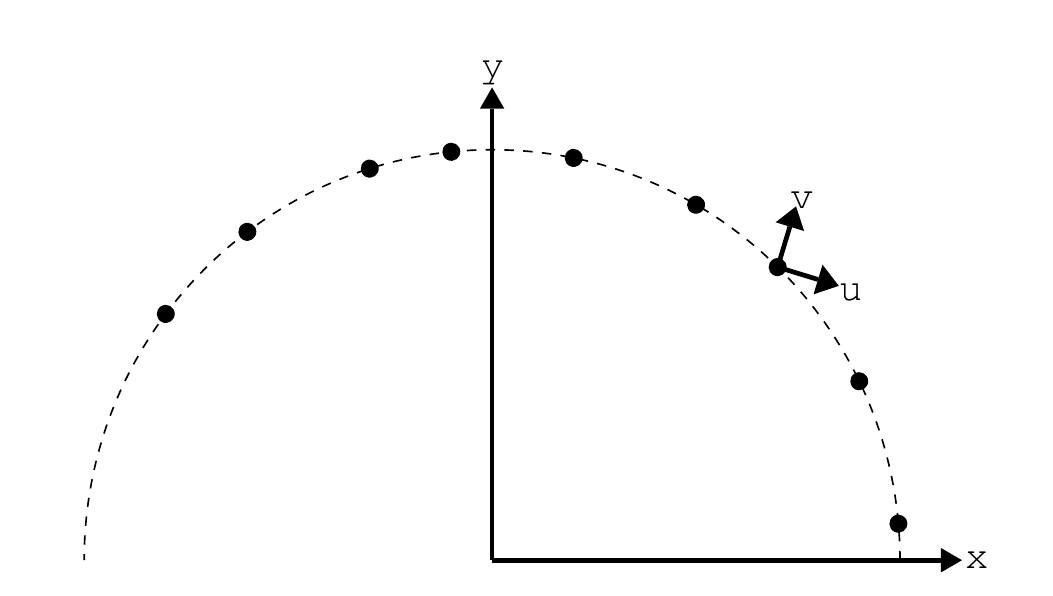
\includegraphics[width=2.5in]{fig-1.png}
  \caption{\(\Omega\) Data Set. The data set is formed by points lying on the upper semicirconference 
  of equation \(x^2 + y^2 = 1\). The ID of \(\Omega\)  is 1. Neverthless PCA yields two
  non-null eigenvalues. The principal components are indicated by \(u\) and \(v\).}
  \label{fig_sim}
\end{figure}

To solve this problem, non-linear algorithms have been proposed. There are two different approaches to get a non-linear PCA: 
an autoassociative approach (Nonlinear PCA) [5,18] and the one based on the use of Mercer kernels (Kernel PCA) [19].
Nonlinear PCA is performed by means of a five-layers neural network. The
neural net has a typical bottleneck structure, shown in Fig. 2. 

\begin{figure}[!t]
  \centering
  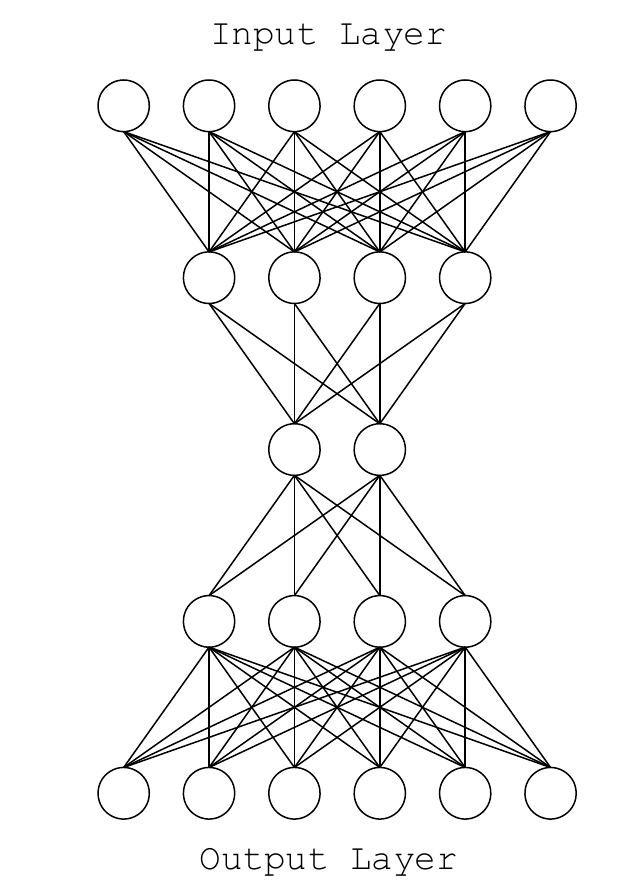
\includegraphics[width=2.5in]{fig-2.png}
  \caption{A Neural Net for Nonlinear PCA}
  \label{fig_sim_2}
\end{figure}


The first (input) and the last (output) layer have the same number of neurons, while the 
remaining hidden layers have less neuron than the first and the last ones. 
The second, the third and the fourth layer are called respectively mapping, bottle-neck and demapping layer. 
Mapping and demapping layers have usually the same number of neurons. The number of the neurons of the bottleneck layer 
provides an ID estimate. The targets used to train Nonlinear PCA are simply the input vector themselves. 
The network is trained with the backpropagation algorithm, minimizing the square error. As optimization algorithm, 
the conjugate-gradient algorithm \cite{Vetterling89} is generally used. 
Though nonlinear PCA performs better than linear PCA in some contexts \cite{Fotheringhame97}, it presents drawbacks when estimating ID. 
As underlined by Malthouse \cite{Malthouse98}, the projections onto curves and surfaces are suboptimal. 
Besides, NLPCA cannot model curves or surfaces that intersect themselves. Kernel PCA consists of making a nonlinear projection of the data set, 
by means of an appropriate positive definite function (Mercer kernel ) \cite{Ressel84} in a new space (Feature Space). 
Then the eigenvalues of the covariance matrix in the Feature Space are computed and ID is given by the number of the non-null eigenvalues. 
The performance of the method is heavily influenced by the kernel choice \cite{Camastra02}. 
Moreover, due to the data noise, last eigenvalues, even if very small, are not null. 
Therefore it is necessary to ignore the eigenvalues whose magnitude is lower than a threshold value that can be only fixed in a heuristic way.
Among projection techniques it is worth mentioning the Whitney reduction network recently proposed by Broomhead and Kirby \cite{Kirby01,Kirby2000}. 
This method is based on Whitney’s concept of good projection [26], namely a projection obtained by means of an injective mapping. 
An injective mapping between two sets \(U\) and \(V\) is a mapping that associate a unique element of \(V\) to each element of \(U\) . As
pointed out in \cite{Kirby01}, finding projections, by means of injective mappings, can be difficult and can sometimes involve empirical considerations.

\subsection{Multidimensional Scaling Methods}
Multidimensional Scaling (MDS) [27,28] methods are projection techniques that tend to preserve the distance among data as much as possible. 
Therefore data that are close in the original data set should be projected in such a way that their projections, 
in the new space (output space), are still close. Among multidimensional scaling algorithms, 
the best known example is MDSCAL, by Kruskal [29] and Shepard [30]. The criterion for the goodness of the projection used by MDSCAL is the \(stress\).

This depends only on the distances between data. When the rank order of the distances in the 
output space is the same as the rank order of the distances in the original data space then the \(stress\) is zero.

Kruskal’s stress \(S_K\) is:
\begin{equation}
  \label{eq_stress_sk}
  S_K =  \Big[\frac{\sum_{i<j}^{[rank(d(x_i, x_j)) - rank(D(x_i, x_j))]^2}}{\sum_{i<j}^{rank(d(x_i, x_j))^2}}\Big]^{\frac{1}{2}}
\end{equation}
  
where \(d(x_i, x_j)\) is the distance between the data \(x_i\) and \(x_j\) and the \(D(x_i, x_j\) is 
the distance of the projections of the same data in the output space. When the stress is zero a perfect projection exists. 
Stress is minimized by iteratively moving the data in the output space from their initially randomly chosen positions 
according to a gradient-descent algorithm.

The intrinsic dimensionality is determined in the following way. The minimum stress for projections of different dimensionalities is computed. 
Then a plot of the minimum stress versus dimensionality of the output space is performed. 
ID is the dimensionality value for which there is a knee or a flattening of the curve. 
Kruskal and Shepard’s algorithm presents a main drawback. The knee or the flattening of the curve could not exists.


\section{Fractal-Based Methods}
Fractal dimension is a statistical quantity that gives an indication of how completely a 
geometric object appears to fill space as one zooms down to finer and finer scales.
It is commonly used in image analysis [33] and chaos theory [41].
Fractal-based techniques are global methods that have been successfully ap-
plied to estimate the attractor dimension of the underlying dynamic system
generating time series [44].
It has also been applied in machine learning and data mining [2], [4]. The idea behind that, is to use the fractal dimension of a data set 
as an estimate of its intrinsic dimension. As defined by Fukunaga [9], if all elements of a 
\(d\)-dimensional data set lie entirely within an \(m\)-dimensional subspace then the data set has an intrinsic dimension of \(m (m < d)\).
From this, it can also be said that only \(m\) independent variables are requried to describe the data set without any information loss.
A number of methods can be used for fractal dimension calculation but the most popular ones are \(Box-Counting\) and \(Correlation\) dimension.

\subsection{Box-Counting Dimension}
The box-counting dimension is a simplified version of Haussdorff dimension [5]. 
The Box-Counting dimension \(D_B\) of a set \(\Omega\) is defined as follows:
if \(v(r)\) is the number of the boxes of size \(r\) needed to cover \(\Omega\), then \(D_B\) is

\begin{equation}
  \label{eq-box-counting}
  D_B = \lim_{r\to 0}\frac{\ln(v(r))}{\ln(\frac{1}{r})}
\end{equation}

Unfortunately, the box-counting dimension can be computed only
for low-dimensional sets because the algorithmic complexity grows
exponentially with the set dimension.

\subsection{Correlational Dimension}

Correlational dimension is a good alternative to the \(Box-Counting\) method. Due to its computational simplicity, the Correlation dimension
is successfully used to estimate the dimension of attractors of dynamical systems.
The Correlation dimension is defined as follows:\\
let \(\Omega = X_1, X_2, X_3,...,X_N\)  be a set of points in \(\mathbb{R}_n\) of cardinality \(N\). 
If the correlation integral \(C_m(r)\) is defined as:


\begin{equation}
  \label{eq-correlational-1}
  C_m(r) = \lim_{N\to \infty}\frac{2}{N(N-1)}\sum_{i=1}^N\sum_{j=i+1}^N I(\parallel X_j - X_i \parallel \leq r) 
\end{equation}

where \(I\) is an indicator function then the Correlation dimension \(D\) of \(\Omega\) is:

\begin{equation}
  \label{eq-correlational-2}
  D = \lim_{r\to 0}\frac{\ln(C_m(r))}{\ln(r)}
\end{equation}

It has been proven [11] that the correlation dimension is a lower bound of the box-counting dimension, but, because of noise, 
the difference between the two is negligible in real applications.  
Some methods [28], [27] have been studied to obtain an optimal estimate for the correlation dimension, but all of these 
techniques work only when the correlation integral assumes the given form in the equation (\ref{eq-correlational-1}).
These methods generally require some heuristics to set the radius r [30].
Therefore, Camastra and Vinciarelli [1S] used the original procedure (GP algorithm) proposed by Grassberger and Procaccia 
that consists of plotting \(\ln(C_m(r))\) versus \(\ln(r)\) and measuring the slope of the linear part of
the curve (\ref{fig_plot_correlation}).

\begin{figure}[!t]
  \centering
  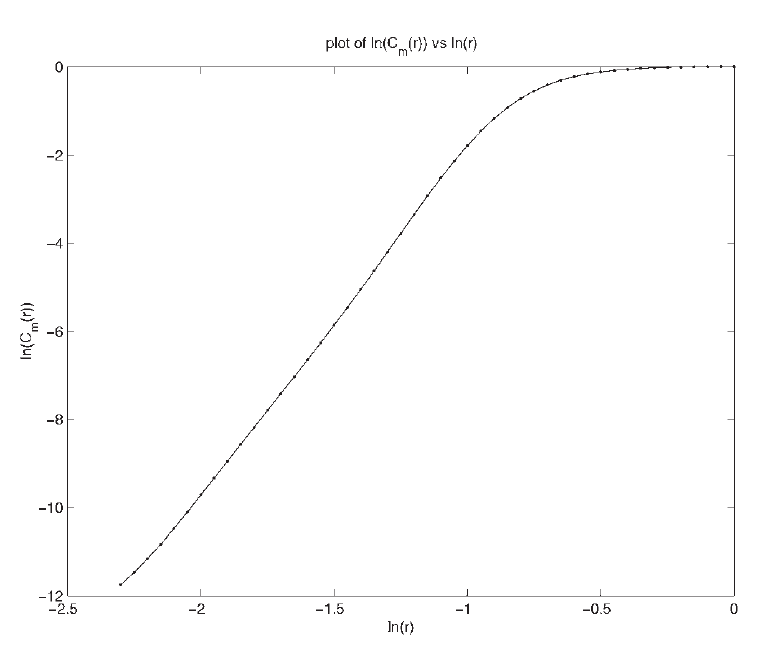
\includegraphics[width=2.5in]{fig-3.png}
  \caption{Plot \(\ln(C_m(r))\) versus \(\ln(r)\)}
  \label{fig_plot_correlation}
\end{figure}

It has been proven [6], [26] that, in order to get an accurate 
estimate of the dimension D, the set cardinality \(N\) has to satisfy the following inequality

\begin{equation}
  \label{eq-correlational-cardinality}
  D = 2\log_{10}N
\end{equation}

Inequality (\ref{eq-correlational-cardinality}) shows that the number \(N\) of data points needed to 
accurately estimate the dimension of a \(D\)-dimensional set is at least \(D^{\frac{10}{2}}\).
But this leads to huge values of \(N\).
The effect of N on the measure of the dimension can be seen in
Table \ref{tbl_effect_of_n}.

\begin{table}[!t]
  \renewcommand{\arraystretch}{2.5}
  \caption{Dependence of the Estimated Correlation Dimension on the Number of Data Points Used (the Actual Dimension of Data is 10)}
  \label{tbl_effect_of_n}
  \centering
  \begin{tabular}{c||c}
  \hline
  \bfseries Points number & \bfseries Estimated dimension\\
  \hline\hline
  1000 & 7.83\\
  2000 & 7.94\\
  5000 & 8.30\\
  10000 & 8.56\\
  30000 & 9.11\\
  100000 & 9.73\\
  \hline
  \end{tabular}
\end{table}
  

This table reports the value of the measures of \(D\) obtained using the GP algorithm over sets of points randomly distributed in
10-dimensional hypercubes (supposed to have \(D = 10\)). The dimension is measured for different values of \(N\) and the error 
with respect to the supposed true dimension is reduced by increasing the number of data points from \(10^3\) to \(10^\frac{10}{2}\ = 10^5\).
To handle this issue and improve the reliability of the measure for low values of \(N\), Camastra and Vinciarelli proposed an empirical procedure 
as described in the below section.

\subsection{Empirical Procedure}

Consider the set \(\Omega\) of cardinality \(N\). The empirical procedure (EP) consists of the following steps:

\begin{enumerate}[\IEEEsetlabelwidth{12)}]
  \item A set \(\Omega'\) , whose ID \(d\) is known, with the same cardinality \(N\) as  \(\Omega\) is created. 
  For instance, \(\Omega'\) could be constituted by \(N\) points randomly generated in a \(d\)-dimensional hypercube.
  
  \item The correlation dimension D of \(\Omega'\) is measured with the GP algorithm.
  
  \item The previous steps are repeated for \(T\) different values of \(d\). 
  The set \(C = \{(d_i, D_i) : i = 1,2,...,T\}\) is obtained.
  
  \item A best-fitting to the points in \(C\) is performed. 
  A plot (reference curve) \(\Gamma\) of \(D\) versus \(d\) is generated (see Fig. \ref{fig_reference_plot}). 
  The reference curve allows to estimate the value of \(D\) when \(d\) is known.
  
  \item The correlation dimension \(D\) of \(\Omega\) is computed and, using \(\Gamma\), 
  the intrinsic dimension of \(\Omega\) can be estimated.
  
\end{enumerate}
  

\begin{figure}[!t]
  \centering
  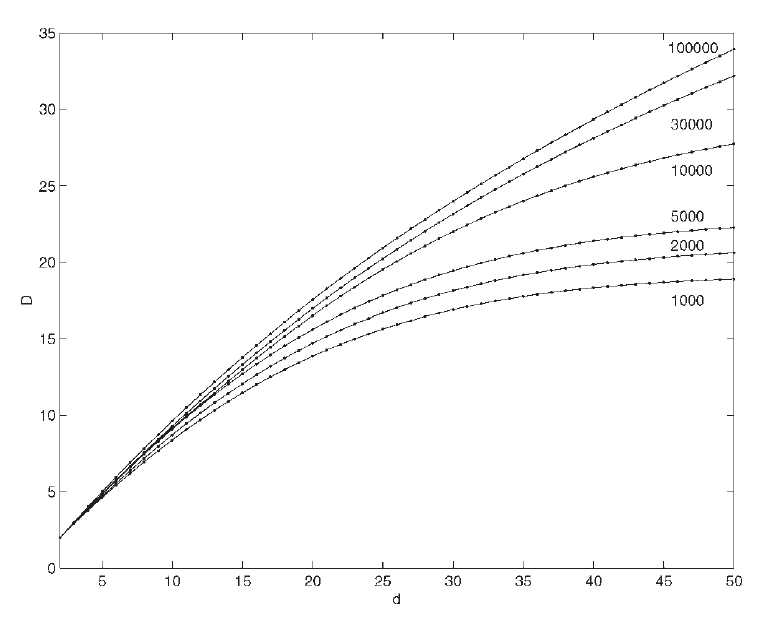
\includegraphics[width=2.5in]{fig-4.png}
  \caption{Reference curves for different values of the cardinality \(N\).}
  \label{fig_reference_plot}
\end{figure}


The above method is based on the following assumptions:
\begin{enumerate}[\IEEEsetlabelwidth{12)}]
  \item \(\Gamma\) depends on \(N\).
  \item Since the GP algorithm gives close estimates for sets of the 
  same dimensionality and cardinality, the dependence of \(\Gamma\) on the \(\Omega'\) sets used for its setup is negligible.
\end{enumerate}

This approach offers the following advantages: it allows one to estimate the ID of high-dimensional data, 
unlike TRN-based method. Moreover, the proposed approach is based on the estimation of a fractal dimension 
and, therefore, allows one to obtain noninteger values. This latter advantage is quite important, 
since, due to the presence of noise, real data can sometimes lie within a \(fractal\)-\(like\) submanifold, whose dimension is usually noninteger.

\subsection{Experimental Results of EP}
The EP was tested by first creating reference curves for different values of the cardinality \(N\), 
then by using each of them to estimate the dimension of data sets of the same cardinality and known dimension.
During our experimentation, the sets \(\Omega\) used for the reference curve setup were formed by randomly generated points in a \(d\)-hypercube. 
A plot was generated for the following cardinality values: 1,000, 2,000, 5,000, 10,000, 30,000, and 100,000. 
Correspondence to each value, a pair \((d, D)\) was calculated for

\begin{equation}
  \label{eq-ep-1}
  d \in \{2, 3, 5, 10, 15, 18, 20, 25, 28, 30, 33, 35, 38, 40, 43, 45, 48, 50\}
\end{equation}

The plot function is estimated by a multilayer-perceptron (MLP) [1]. 
Its structure was set up by means of the \(Bayesian information criterion\) [25].
The resulting reference curves can be seen in Fig. \ref{fig_reference_plot}
In order to test the method, several sets (with cardinalities corresponding to the values indicated above) were created 
composed of random points generated in hypercubes in spaces with dimension 8 and 23. These sets were assumed to have ID 8 and 23, 
respectively, and were not used to generate the reference curves \(\Gamma\).
Following the procedure described in Section 4, the GP algorithm was first applied for each set, then the plot  \(\Gamma\) 
corresponding to the same cardinality as the set being measured was used to compute the ID. The results are reported in Table \ref{tbl_gp_ep_comp}.

\begin{table}[!t]
  \renewcommand{\arraystretch}{2.5}
  \caption{ID Estimation by the GP Algorithm and EP of 8-Dimensional and 23-Dimensional Data Sets}
  \label{tbl_gp_ep_comp}
  \centering
  \begin{tabular}{c||c||c||c||c}
  \hline
  \bfseries Points & \bfseries GP (d=8)\ & \bfseries EP (d=8) & \bfseries GP (d=23) & \bfseries EP (d=23)\\
  \hline\hline
  1000 & 6.83 & 7.86 & 14.99 & 22.95\\
  2000 & 6.94 & 7.75 & 15.76 & 22.48\\
  5000 & 7.42 & 7.98 & 17.09 & 23.21\\
  10000 & 7.51 & 8.20 & 18.04 & 22.43\\
  30000 & 7.65 & 8.13 & 19.10 & 23.20\\
  100000 & 7.83 & 8.03 & 19.78 & 23.24\\
  \hline
  \end{tabular}
\end{table}


The table shows the dimension estimation obtained with the GP algorithm and with the empirical procedure proposed here.
Indeed, a remarkable improvement is obtained when the cardinality is low. Afterwards, in order to validate the EP procedure, 
the data set \(A\) [14] and \(D\) [23] of the Santa Fe time series competition were considered.
Data Set \(A\) is a real data time series generated by a Lorenz-like chaotic system, implemented by \(NH_3-FIR\) lasers. 
The data set D is a synthetic time series generated by a particle motion, simulated on a computer, with nine freedom degrees. 
The goal of the experimentation was to estimate, with the GP procedure, the attractor dimension of time series \(A\) and \(D\).

In order to estimate the attractor dimension, they used the method of delays [17], [22] to the data set \(A\), 
considering its first 1,000, 2,000, 5,000, 10,000 points. The results, obtained with the GP and EP algorithms, are reported in Table \ref{tbl_gp_ep_santa}. 



\begin{table}[!t]
  \renewcommand{\arraystretch}{2.5}
  \caption{Estimation of the Attractor Dimension of the Series D and A of Santa Fe Competition}
  \label{tbl_gp_ep_santa}
  \centering
  \begin{tabular}{c||c||c||c||c}
  \hline
  \bfseries Points & \bfseries GP (D)\ & \bfseries EP (D) & \bfseries GP (A) & \bfseries EP (A)\\
  \hline\hline
  1000 & 7.54 & 8.84 & 2.00 & 2.01\\
  2000 & 7.87 & 8.90 & 2.01 & 2.02\\
  5000 & 8.13 & 8.83 & 2.03 & 2.03\\
  10000 & 8.25 & 9.09 & 2.03 & 2.03\\
  30000 & 8.48 & 9.07\\
  \hline
  \end{tabular}
\end{table}


Since the value of the fractal dimension of the attractor of Lorenz’s system is approximately 2:06, the result can be considered satisfactory.
They then applied the method of delays to the data set D, considering the first 1,000, 2,000, 5,000, 10,000, 30,000 points. 
The results, with GP and EP, are shown in Table \ref{tbl_gp_ep_santa}. Since the system that generated the data \(D\) has 9 degrees of freedom, 
the result can be considered particularly satisfactory.


% An example of a floating figure using the graphicx package.
% Note that \label must occur AFTER (or within) \caption.
% For figures, \caption should occur after the \includegraphics.
% Note that IEEEtran v1.7 and later has special internal code that
% is designed to preserve the operation of \label within \caption
% even when the captionsoff option is in effect. However, because
% of issues like this, it may be the safest practice to put all your
% \label just after \caption rather than within \caption{}.
%
% Reminder: the "draftcls" or "draftclsnofoot", not "draft", class
% option should be used if it is desired that the figures are to be
% displayed while in draft mode.
%
%\begin{figure}[!t]
%\centering
%\includegraphics[width=2.5in]{myfigure}
% where an .eps filename suffix will be assumed under latex, 
% and a .pdf suffix will be assumed for pdflatex; or what has been declared
% via \DeclareGraphicsExtensions.
%\caption{Simulation Results}
%\label{fig_sim}
%\end{figure}

% Note that IEEE typically puts floats only at the top, even when this
% results in a large percentage of a column being occupied by floats.


% An example of a double column floating figure using two subfigures.
% (The subfig.sty package must be loaded for this to work.)
% The subfigure \label commands are set within each subfloat command, the
% \label for the overall figure must come after \caption.
% \hfil must be used as a separator to get equal spacing.
% The subfigure.sty package works much the same way, except \subfigure is
% used instead of \subfloat.
%
%\begin{figure*}[!t]
%\centerline{\subfloat[Case I]\includegraphics[width=2.5in]{subfigcase1}%
%\label{fig_first_case}}
%\hfil
%\subfloat[Case II]{\includegraphics[width=2.5in]{subfigcase2}%
%\label{fig_second_case}}}
%\caption{Simulation results}
%\label{fig_sim}
%\end{figure*}
%
% Note that often IEEE papers with subfigures do not employ subfigure
% captions (using the optional argument to \subfloat), but instead will
% reference/describe all of them (a), (b), etc., within the main caption.


% An example of a floating table. Note that, for IEEE style tables, the 
% \caption command should come BEFORE the table. Table text will default to
% \footnotesize as IEEE normally uses this smaller font for tables.
% The \label must come after \caption as always.
%
%\begin{table}[!t]
%% increase table row spacing, adjust to taste
%\renewcommand{\arraystretch}{1.3}
% if using array.sty, it might be a good idea to tweak the value of
% \extrarowheight as needed to properly center the text within the cells
%\caption{An Example of a Table}
%\label{table_example}
%\centering
%% Some packages, such as MDW tools, offer better commands for making tables
%% than the plain LaTeX2e tabular which is used here.
%\begin{tabular}{|c||c|}
%\hline
%One & Two\\
%\hline
%Three & Four\\
%\hline
%\end{tabular}
%\end{table}


% Note that IEEE does not put floats in the very first column - or typically
% anywhere on the first page for that matter. Also, in-text middle ("here")
% positioning is not used. Most IEEE journals use top floats exclusively.
% Note that, LaTeX2e, unlike IEEE journals, places footnotes above bottom
% floats. This can be corrected via the \fnbelowfloat command of the
% stfloats package.



\section{Conclusion}
The conclusion goes here.





% if have a single appendix:
%\appendix[Proof of the Zonklar Equations]
% or
%\appendix  % for no appendix heading
% do not use \section anymore after \appendix, only \section*
% is possibly needed

% use appendices with more than one appendix
% then use \section to start each appendix
% you must declare a \section before using any
% \subsection or using \label (\appendices by itself
% starts a section numbered zero.)
%


\appendices
\section{Proof of the First Zonklar Equation}
Appendix one text goes here.

% you can choose not to have a title for an appendix
% if you want by leaving the argument blank
\section{}
Appendix two text goes here.


% use section* for acknowledgement
\section*{Acknowledgment}


The authors would like to thank...


% Can use something like this to put references on a page
% by themselves when using endfloat and the captionsoff option.
\ifCLASSOPTIONcaptionsoff
  \newpage
\fi



% trigger a \newpage just before the given reference
% number - used to balance the columns on the last page
% adjust value as needed - may need to be readjusted if
% the document is modified later
%\IEEEtriggeratref{8}
% The "triggered" command can be changed if desired:
%\IEEEtriggercmd{\enlargethispage{-5in}}

% references section

% can use a bibliography generated by BibTeX as a .bbl file
% BibTeX documentation can be easily obtained at:
% http://www.ctan.org/tex-archive/biblio/bibtex/contrib/doc/
% The IEEEtran BibTeX style support page is at:
% http://www.michaelshell.org/tex/ieeetran/bibtex/
\bibliographystyle{IEEEtran}
% argument is your BibTeX string definitions and bibliography database(s)
%\bibliography{IEEEabrv,../bib/paper}
%
% <OR> manually copy in the resultant .bbl file
% set second argument of \begin to the number of references
% (used to reserve space for the reference number labels box)
\bibliography{agrosy} 

% biography section
% 
% If you have an EPS/PDF photo (graphicx package needed) extra braces are
% needed around the contents of the optional argument to biography to prevent
% the LaTeX parser from getting confused when it sees the complicated
% \includegraphics command within an optional argument. (You could create
% your own custom macro containing the \includegraphics command to make things
% simpler here.)
%\begin{biography}[{\includegraphics[width=1in,height=1.25in,clip,keepaspectratio]{mshell}}]{Michael Shell}
% or if you just want to reserve a space for a photo:

%\begin{IEEEbiography}{Jane Doe}
%Biography text here.
%\end{IEEEbiography}

% if you will not have a photo at all:
%\begin{IEEEbiographynophoto}{John Doe}
%Biography text here.
%\end{IEEEbiographynophoto}


% You can push biographies down or up by placing
% a \vfill before or after them. The appropriate
% use of \vfill depends on what kind of text is
% on the last page and whether or not the columns
% are being equalized.

%\vfill

% Can be used to pull up biographies so that the bottom of the last one
% is flush with the other column.
%\enlargethispage{-5in}



% that's all folks
\end{document}


